\section{\gls{T11} Retrospective}

In our retrospective of sprint 3 we discussed how the sprint went and how the points from last sprint went.

\subsection{Issues from previous sprint}

We still had issues with getting the chapters in the report. However, we did not experience the same problems with understanding how much work that had been done as in Sprint 2.

Since last sprint, the merge process have run smoother. This is likely a result of loosening the rules a little, and the team members getting more used to the merging process.

In Sprint 3 we were better at answering each other when we worked from home, but we still had some problems with this.

During Sprint 3 we tried to switch the roles so the members that did a lot of work on the report in Sprint 2 worked on the \gls{giraf} user stories and vise versa. We had some problems with this because of two things. The first thing was that the user stories we got were either blocked for a long time or were annulled, and we had a difficult time getting new work when we wanted. The second thing were that the members that usually worked on the code got asked to help other groups a lot of the time. This resulted in the members having approximately the same roles in this sprint as in the last. This also relate to the final point of the previous retrospective because we were unsuccessful in redirecting other groups to \gls{POT}.

\subsection{Issues this sprint}

We did not meet at the university as much during sprint 3 because of the easter holiday, and therefore we did not have a lot to talk about in this retrospective. There were however still one significant issue.

\begin{figure}[ht]
    \centering
    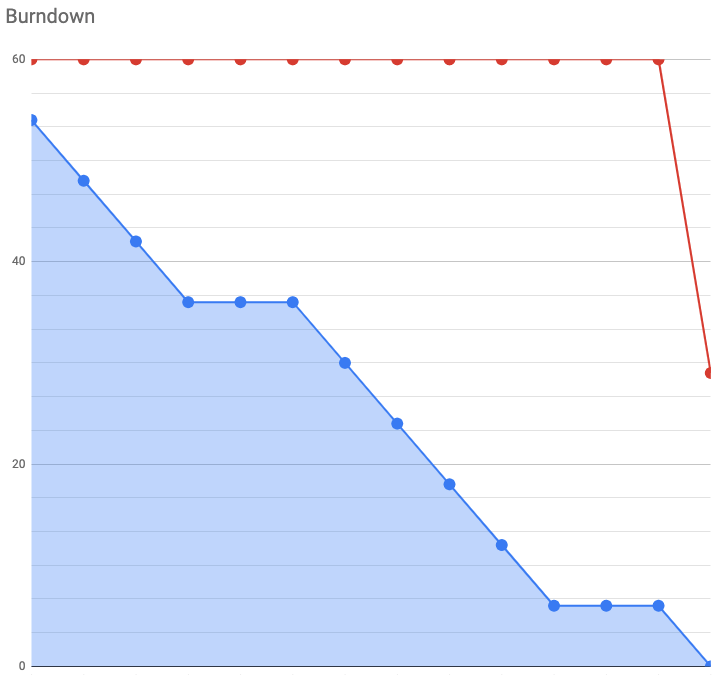
\includegraphics[width=0.5\textwidth]{figures/burndown.png}
    \caption{The burndown chart for sprint 3, blue meaning expected, red meaning actual burnrate.}
    \label{fig:burndown-chart}
\end{figure}

One issue was our planning. We had made a sprint backlog in the beginning of the sprint where we put tasks we wanted to do during the sprint. We made a burndown chart for the backlog, which we can see in \autoref{fig:burndown-chart}. This showed two things. The first thing was that we only finished about half the tasks we planned. This shows unrealistic planning, which we want to avoid in Sprint 4. We also noticed that almost all the tasks we had done finished within the last days of the sprint, rather than during the sprint. We discussed this and concluded that we had finished most tasks during the sprint but we had not reviewed them before the end. We decided to be better at reviewing the tasks quickly after they are finished.

\subsection{Things that went well}
Most of our collaboration were successful. In this sprint we were more used to working together than before. We are also good at communicating issues and there is a high degree of respect in the group. Although we have small problems with our planning, we do a lot of work. Since the last sprint we have only gotten better at working together.
